%!TEX root = ../thesis.tex
%*******************************************************************************
%****************************** Fourth Chapter *********************************
%*******************************************************************************

\chapter{Identifying dynamic eQTL effects during iPSC differentiation using scRNA-seq}

As outlined in section 1.2, human \gls{ipsc}s and cells derived from them have proven to be an excellent system to study cell fate decisions in early human development \textit{in vitro}, which cannot be studied \textit{in vivo}.
So far, experiments have been limited to a handful of individuals (ref) or have focused on one single time point \cite{kilpinen2017common, schwartzentruber2018molecular}, thus the extent to which development varies from individual to individual, and the role played by common genetic variants during the process remains largely unexplored.
Here, we combine human iPS cell lines from over one hundred donors, a pooled experimental design, and single-cell RNA-sequencing to study population variation during differentiation to a definitive endoderm fate. 
We identify molecular markers that are predictive of differentiation efficiency of individual \gls{ipsc} lines, and exploit heterogeneity in the genetic background across individuals to map hundreds of expression quantitative trait loci that influence expression dynamically during differentiation and across cellular contexts.\\

\newpage

\begin{Comment2}
\hspace{-3mm}\textbf{Contributions} \\
This work was a joint effort of the Stegle, Marioni and Vallier labs. 
In particular, the data was generated by Ludovic Vallier’s lab at the Sanger Institute, and the experiments were led by Mariya Chhatriwala, who also contributed to the interpretation of the results. 
All cell lines used are from the \gls{hipsci} project.
The statistical methods and analyses described in this chapter were co-supervised by Oliver Stegle and John Marioni. 
I processed the data and performed lengthy quality control in collaboration with Davis McCarthy. 
I developed and implemented the statistical methods for eQTL mapping, while
Daniel Seaton performed the ASE analysis.
The code for processing, analysing and plotting the data is open source and freely accessible here: https://github.com/single-cell-genetics/singlecell\_endodiff\_paper.\
Daniel Seaton, John Marioni, Oliver Stegle and I wrote the manuscript. 
The paper \cite{cuomo2020single} is available at https://www.nature.com/articles/s41467-020-14457-z and has been published as:\\

Anna S.E. Cuomo*, Daniel D. Seaton*, Davis J. McCarthy*, Iker Martinez, Marc Jan Bonder, Jose Garcia-Bernardo, Shradha Amatya, Pedro Madrigal, Abigail Isaacson, Florian Buettner, Andrew Knights, Kedar Nath Natarajan, the Hipsci Consortium, Ludovic Vallier, John C. Marioni, Mariya Chhatriwala, Oliver Stegle. Single-cell RNA-sequencing of differentiating iPS cells reveals dynamic genetic effects on gene expression. \textit{Nature Communications}, 2020, (* equal contribution)

\end{Comment2}

\newpage

\section{Introduction}

As highlighted in section 1.2, the early stages of embryogenesis involve dramatic and dynamic changes in cellular states. 
As cells go from a pluripotent state, where they still have the potential to differentiate to all cell types, to committing to a specific cell fate, many molecular programs and mechanisms are activated and tightly regulated.
Our understanding of such mechanisms in humans is still only partial, yet a lot has been learnt in model organisms including fruit flies, Zebrafish, and mice. 
For obvious (ethical) reasons, such mechanisms cannot be studied \textit{in vivo} for humans. 
There exist a few studies that use human embryonic stem cells (hESCs) but the data is hard to access, and often limited to a narrow time frame within development (section 1.2). \\

Human induced pluripotent stem cells (h-iPSCs) and iPS-derived cells offer great potential to interrogate cell types and states that are challenging if not impossible to access in human, \textit{in vivo} \cite{kilpinen2017common}.
In particular, the study of early development can be mimicked \textit{in vitro} using iPS-derived differentiation protocols. 
This highly controlled setup allows us to sample at tight intervals in time and provides a unique opportunity to study the dynamic effect of common genetic variants on gene expression regulation during early development.
However, \gls{ipsc} differentiation protocols are challenging to apply in practice: most protocols generate much more diversity than intended in terms of cell types (ref). \cite{bock2011reference}
Additionally, extensive batch to batch as well as line-to-line heterogeneity has been observed (refs) \cite{schwartzentruber2018molecular}. 
Finally, the protocols are lengthy and hard to scale leading to limited throughput. 
In this study, we employed different strategies to combat some of these issues.\\ 

First, the single cell RNA-seq readout allows cellular heterogeneity to be assessed in a continuous manner across development.
Second, our pooling strategy - where we differentiate cells coming from 4 to 6 donors in the same pool - allows us to increase throughput to population-scale and allows us to control for technical batch to batch variation, enhancing the ability of inter line comparisons.
Finally, we selected a short and efficient protocol, which models an extremely well understood developmental process thus acting as a proof of principle study.\\

In this study, we differentiate iPS cell lines from 125 donors towards definitive endoderm, one of the three germ layers (alongside the ectoderm and the mesoderm). 
This is a short (three days) and well-established protocol \cite{hannan2013production} that is the basis for longer differentiation experiments toward disease-relevant tissues such as the gut, the pancreas and the lungs.
The generation of population-scale collections of differentiating human \gls{ipsc}s allows the study of inter-individual variability effects, which is key as cellular reprogramming becomes an increasingly used tool in molecular medicine.

\section{Single-cell RNA sequencing of differentiating human iPS cells}
\subsection{Experimental design}

We adopt a pooled experimental design.
Each differentiation experiment (hereon simply "experiment") consisted of iPS cells from 4 to 6 distinct cell lines from the \gls{hipsci} collection.
We retain data from a total of 28 experiments.
Cells were collected at four time points, at iPS stage (day0) and then after 24, 48 and 72 hours post initiation (day1, day2, day3); their transcriptomes were assayed using full-length RNA sequencing (using the SmartSeq2 technology \cite{picelli2013smart}).
Additionally, we recorded the expression of two selected cell surface markers using FACS, a pluripotency marker and a definitive endoderm marker, respectively (Tra-1-60 and CXCR4).
Imputed genotypes were also available for all lines through \gls{hipsci}.

\begin{figure}[h]
\centering
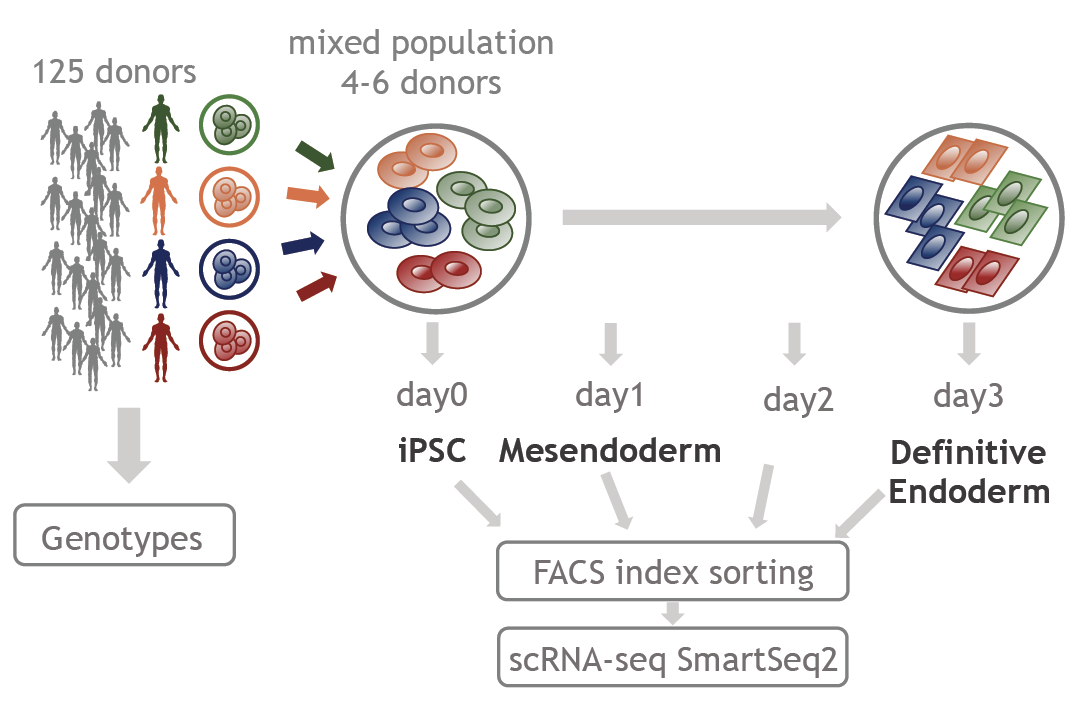
\includegraphics[width=12cm]{Chapter4/Fig/endodiff_experimental_design.png}
\caption[\textbf{Experimental Design}]{\textbf{Experimental Design}.\\
Human \gls{ipsc} lines from 125 unrelated donors were differentiated to definitive endoderm using a pooled design, where cells from 4 to 6 lines were grown and differentiated together.
Cells were collected prior to differentiation (day0) and every 24 hours along differentiation to definitive endoderm (day1, day2, day3).
Cells at day0 are expected to be pluripotent; cells at day1 are considered to be bipotent for either mesoderm or endoderm (mesendoderm); by day3, cells should have reached a definitive endoderm state.
At each time point, cells are FACS sorted and sequenced using the SmartSeq2 technology.
Imputed genotypes were available for all lines.}
\label{fig:endodiff_experimental_design}
\end{figure}

\subsection{Data processing and QC}

\subsubsection{Demultiplexing donors from pooled experiments} 

The pooled experimental design means that cells from multiple donors are differentiated together in the same experiment. 
To be able to link the genetic background of an individual with their transcriptional profile we need to map the cells back to their donor of origin, without the use of any barcode.
Indeed, we find that for the large majority of cells the RNA-seq reads map to a sufficient number of common genetic variants for us to reliably assign each cell to its original donor.

In particular, assignment of cells to donors was performed using Cardelino \cite{mccarthy2020cardelino}. 
Briefly, Cardelino estimates the posterior probability of a cell originating from a given donor based on common genetic variants in scRNA-seq reads, while employing a beta binomial-based Bayesian approach to account for technical factors (e.g. differences in read depth, allelic drop-out, and sequencing accuracy). 
For this assignment step, we considered a larger set of n = 490 \gls{hipsci} lines with genotype information, which included the 126 lines used in this study. 
A cell was assigned to a donor if the model identified the match with posterior probability >0.9, requiring a minimum of 10 informative variants for assignment. 
Cells for which the donor identification was not successful were not considered further.
Across the full dataset 99\% of cells that passed RNA QC steps (below) were successfully assigned to a donor.\\

% \subsubsection{Plate swaps}

In some cases, unexpected donor assignment (where several cells from one experiment were found to be assigned to none of the 4-6 donors used in that experiment) allowed us to identify (and correct) plate swaps that happened in the lab (fig), without losing any data.

\subsubsection{scRNA-seq feature quantification and quality control}

Single cell profiles were obtained using the SmartSeq2 technology \cite{picelli2013smart}. 
This is a plate-based technology that involves single cells being sorted into 384 independent wells on a plate. 
Obtained reads are then mapped to a human genome reference using STAR \cite{dobin2013star}. 
Gene-level expression quantification was performed using Salmon \cite{patro2017salmon}. 
Briefly, Salmon quantifies transcript (rather than gene-) level expression levels, similar to Kallisto \cite{bray2016near}.
Then, such values are summarised at a gene level (estimated \gls{cpm}).
We performed \gls{qc} of scRNA-seq profiles following a widely used pipeline using Bioconductor (ref) packages scater \cite{mccarthy2017scater} and scran, implemented in R (refs).  
In particular, cells were retained for downstream analyses if they had at least 50,000 counts from endogenous genes, at least 5,000 genes with non-zero expression, less than 90\% of counts came from the 100 highest-expressed genes, less than 15\% of reads mapping to mitochondrial (MT) genes, they had a Salmon mapping rate of at least 60\%, and if the cell was successfully assigned to a donor (add figure similar to Supplementary Figure 20). 


\subsubsection{Flow cytometry}

Additionaly, dead cells as identified based on 7AAD using fluorescence-activated cell sorter (FACS) staining were discarded. 
FACS data was analysed using the openCyto package, implemented in R \cite{finak2014opencyto}. 

% Single cells/Doublets

The success of the differentiation protocol was assessed using expression of two protein surface markers Tra-1-60 and CXCR4 which are markers of pluripotency and definitive endoderm stage, respectively. 
Note that cells were not gated using the two markers, we simply recorded their expression (similar to Supplementary Figure 3/4). 

\subsubsection{scRNA-seq processing}

SmartSeq2 data does not include \gls{umis} which can help normalisation by providing a comparable measure of the amount of reads sequenced per cell. 
In the absence of \gls{umis}, we can borrow information from cells with similar total number of reads and correct for overall library size. 
Such size factor normalisation of counts was performed using scater \cite{mccarthy2017scater}. 

Expressed genes with an HGNC symbol were retained for analysis, where expressed genes in each batch of samples were defined based on (i) raw count >100 in at least one cell prior to QC and (ii) average log2(CPM+1) >1 after QC. 
Normalised CPM data were log transformed (log2(CPM+1)) for all downstream analyses. 
The joint dataset was investigated for outlying cell lines or experimental batches, which identified no clear groups of outlying cells. 

As a final QC assessment, we considered possible differences between cell lines from healthy and diseased donors. 
In particular, a subset of 11 cell lines were derived from neonatal diabetes patients, and differentiated together with cell lines from healthy donors across 7 experiments (out of 28). 
There was no detectable difference in differentiation capacity between healthy and neonatal diabetes lines in these experiments (p value > 0.05), and cells from both sets of donors overlapped in principal component space. 
Thus, we included cells from all donors in our analyses irrespective of disease state.
% The final merged and QC’ed dataset consisted of 36,044 cells with expression profiles for 11,231 genes.
(possibly add workflow figure, similar to Suppl.Fig.5)


% \section{Results}

\section{Data overview}

%  We considered a panel of well-characterized human \gls{ipsc} lines derived from 125 unrelated donors from the \gls{hipsci} collection \cite{kilpinen2017common}. 
%  In order to increase throughput and mitigate the effects of batch variation, we exploited a novel pooled differentiation assay, combining sets of four to six lines in one well prior to differentiation (28 differentiation experiments performed in total; hereon “experiments”; Fig. 1A). 
%  Cells were collected at four differentiation time points (iPSC; one, two and three days post initiation - hereon day0, day1, day2 and day3) and their transcriptomes were assayed using full-length RNA-sequencing (Smart-Seq2 \cite{picelli2013smart}) alongside the expression of selected cell surface markers using FACS (TRA-1-60, CXCR4). 
 Following quality control (QC), 36,044 cells were retained for downstream analysis, across which 11,231 genes were expressed.
 Exploiting the observation that each cell line’s genotype acts as a unique barcode, we demultiplexed the pooled cell populations, enabling identification of the cell line of origin for each cell (similar to \cite{kang2018multiplexed}). 
 At each time point, cells from between 104 and 112 donors were captured, with each donor being represented by an average of 286 cells (after QC). 
 The success of the differentiation protocol was validated using canonical cell-surface marker expression: consistent with previous studies \cite{chu2016single}, an average of 72\% of cells were TRA-1-60(+) in the undifferentiated state (day0) and an average of 49\% of cells were CXCR4(+) three days post differentiation (day3).

\subsection{Sources of variation} 

To identify the main sources of variation in our dataset we performed variance component analysis across all genes, using a linear mixed model.
Variance component analysis revealed the time point of collection as the main source of variation, followed by the cell line of origin and the experimental batch. 

Next, we performed \gls{pca} on our dataset.
To do, we first identified the top 500 \gls{hvgs} defined as the most variable genes given a mean-variance trend calculated across all genes, using trenVar as implemented in the R package scran.

Consistent with the results from the variance component analysis, the first principal component (PC1) was strongly associated with differentiation time (Fig. 1C), motivating its use to order cells by their differentiation status (hereafter “pseudotime”, Fig. 1C).
Pseudotime inference is a common step in scRNA-seq data analysis and it ..
In this case, the nature of the short and linear differentiation process of our data (i.e. iPSC $\rightarrow$ mesendoderm $\rightarrow$ definitive endoderm) meant that PC1 nicely captured the differentiation trajectory.

For comparison, we did apply alternative pseudotime inference methods, which yielded similar orderings (fig).
 
Further validation of our inferred pseudotime was provided by the temporal expression dynamics of known marker genes that characterise endoderm differentiation which was captured by our ordering of cells as expected (fig).



% \subsubsection{Map to gastrulation atlas??}

\section{eQTL maps iPSCs, mesendo, defendo}

As we discussed in Chapter 3, the early stages of human development involve dynamic changes in cellular states and quick cell fate decisions. 
However, the extent to which an embryo’s genetic background influences this process has only been determined in a small number of special cases linked to rare large-effect variants that cause developmental disorders. 
This lack of information is critical - it can provide a deep understanding of how genetic heterogeneity is tolerated in normal development, when controlling the expression of key genes is vital. 
Combining single cell profiling and genetic variation of enough individuals can facilitate assessment of the molecular impact of genetic variability in a continuous manner across early human development.\\
 
We have deep genotype information for all of our 125 samples, so this study allows discovery of eQTL at various stages of early human development. 
This was partly motivated by the observation that a substantial fraction of variability in gene expression was explained by cell-line effects (Fig. XX).

\subsection{Developmental stages}
% rephrase and bulk up

To be able to exploit methods similar to those described in the previous section (chapter 3) to map eQTL, we must first define homogeneous populations of cells.
Exploiting the previously described markers of differentiation progress and our inferres pseudotime, we assigned 28,971 cells (about $\sim$80\% of all cells) to one of three canonical stages of endoderm differentiation: \gls{ipsc}, mesendoderm (mesendo) and definitive endoderm (defendo) (Fig. 1C). 
A smaller fraction of cells (N = 7,073) could not be confidently assigned to a canonical stage of differentiation; these cells were heavily enriched for those collected at day2, when rapid changes in molecular profiles are expected, reflecting a transitional population of cells.

Using these  developmental stages and methods similar to those described above, we mapped eQTL in each of the \gls{ipsc}, mesendo and defendo populations, yielding 1,833, 1,702 and 1,342 eGenes, respectively. 

\subsection{Mapping eQTL}

Briefly, for each donor, experiment, and differentiation stage, we quantified each gene’s average expression level\footnote{This approach is similar to the "total mean" described in chapter 3, except that the aggreagation is done at the experiment level rather than the sequencing run level}, before using a linear mixed model to test for \textit{cis} eQTL, adapting approaches used for bulk RNA-seq profiles (+ and - 250 kb, MAF >5\% \cite{kilpinen2017common}).

For comparison, we also performed eQTL mapping in cells collected on day1 and day3 — the experimental time points commonly used to identify cells at mesendo and defendo stages \cite{hannan2013production}.
% following needs rephrasing (identical to paper now)
Interestingly, this approach identified markedly fewer eGenes (1,181 eGenes at day1, and 631 eGenes at day3), demonstrating the power of using the single-cell RNA-seq profiles to define relatively homogeneous differentiation stages in a data-driven manner. 
Notably, this observation did not merely reflect differences in the number of cells or donors considered.\\

% rephrase all of the below

Profiling multiple stages of endoderm differentiation allowed us to assess at which stage along this process individual eQTL can be detected as well as the level of sharing of genetic signal across time. 
We observed substantial regulatory and transcriptional remodelling upon iPS differentiation to definitive endoderm, with over 30\% of eQTL being specific to a single stage (Fig. 2a, c), where we considered the pairwise replication of eQTL to define stage-specific effects (nominal p value < 0.05 and consistent effect direction). 
Importantly, we note that stage-specificity of eQTL was not significantly explained by stage-specific gene expression (Supplementary Fig. 12). 
Our differentiation time course covers developmental stages that have never before been accessible to genetic analyses of molecular traits. 
Consistent with this, 349 of our eQTL variants at the mesendo and defendo stages have not been reported in either a recent iPSC eQTL study based on bulk RNA-seq \cite{mirauta2018population}, or in a compendium of eQTL identified from 49 tissues as part of the GTEx project \cite{gtex2017genetic} (linkage disequilibrium with lead variants in GTEx, LD: $r^2<0.2$; Methods; Supplementary Data 3).\\

In addition to these eQTL, we identified lead switching events for 155 eGenes. 
Those are two distinct variants for the same gene that are identified as lead eQTL at different stages of differentiation (at LD: $r^2<0.2$; for example iPSC and defendo in Fig. 2d; Methods). 
To investigate the potential regulatory role of such variants, we examined whether the corresponding genetic loci also featured changes in histone modifications during differentiation. 
Specifically, we used ChIP-Sequencing to profile five histone modifications associated with promoter and enhancer usage (H3K27ac, H3K4me1, H3K4me3, H3K27me3, and H3K36me3) in hESCs that were differentiated towards endoderm (using the same protocol employed above) and measured at equivalent time points (i.e. day0, day1, day2, day3; Methods). 
Intriguingly, for 20 of the lead switching events, we observed corresponding changes in the epigenetic landscape (stage-specific lead variants overlap with stage-specific changes in histone modification status), suggesting a direct mode of action (Fig. 2d).

\section{Dynamic eQTL across iPSC differentiation to endoderm}

The availability of large numbers of cells per donor across a continuous differentiation trajectory from pluripotent stage to definitive endoderm enabled the analysis of dynamic changes of eQTL strength at fine-grained resolution. 

\subsection{Running average}

First, for visualization purposes, we used a sliding-window approach. 
Because we need a rather large amount of cells to reliably estimate expression abundance for each of our individuals, we slide a window containig 25\% of the cells along pseudotime by a step of 2.5\% cells.
In each window, we considered average expression quantifications and estimate genetic effects using eQTL mapping, essentially performing the same analysis we perform in three developmental stages in each window (4.5). 

We focused on the joint set of 4,422 eQTL lead variants (4,470 SNP-gene pairs) discovered at the iPSC, mesendo, and defendo stages and explored how they were modulated by developmental time.

In parallel, we reassessed each eQTL in each window taking advantage of the full length transcript sequencing to measure allele-specific expression (ASE).
Here, in each window, we quantified the deviation from 0.5 of the expression of the minor allele at the eQTL (ratio of reads phased to eQTL variants, Methods). 
Notably, ASE can be quantified in each cell and is independent of expression level, thus mitigating technical correlations between differentiation stage and genetic effect estimates.

Both methods result in a measure of the varying strength of genetic effects along development, or genetic effect dynamics. 
Reassuringly, the two approaches were highly consistent across pseudotime (Fig. 3a, Supplementary Fig. 13).\\

\subsection{Interaction tests}

\subsubsection{Allele specific expression}

To formally test for eQTL effects that change dynamically across differentiation (dynamic QTL), we tested for associations between pseudotime and the genetic effect size using a linear model:

\begin{equation}
    ASE = pseudotime + pseudotime^2 + \epsilon
\end{equation}

(genetic effect defined based on ASE at the level of single cells; likelihood ratio test, considering linear and quadratic pseudotime), uncovering a total of 899 time dynamic eQTL (out of the joint set of 4422 eQTL across all stages; FDR<10\%; Methods), including a substantial fraction of eQTL that were not stage-specific (Supplementary Data 3). 
This complements our earlier analysis based on discrete differentiation stages, which identified substantial stage-specific effects (Fig. 2a,c), by identifying subtle changes in the relationship between genotype and phenotype during differentiation. 
To further explore this set of genes, we clustered eQTL jointly based on the relative gene expression dynamics (global expression changes along pseudotime, quantified in sliding windows as above, Methods), and on the genetic effect dynamics (Fig. 3a; Methods). 
This identified four basic dynamic patterns (Fig. 3b): decreasing early (cluster A), decreasing late (cluster B), transiently increasing (cluster C), and increasing (cluster D). 
As expected, stage-specific eQTL were grouped together in particular clusters (e.g. defendo specific eQTL in cluster D; Supplementary Fig. 14). 
Notably, the gene expression dynamics and the eQTL dynamics tended to be distinct, demonstrating that gene expression level is not the primary mechanism governing variation in genetic effects. 
In particular, genetic effects were not most pronounced when gene expression was high (Fig. 3c, d, Supplementary Fig. 15).\\

Distinct combinations of expression and eQTL dynamics result in different patterns of allelic expression. 
This is illustrated by the mesendoderm-specific eQTL for \textit{VAT1L}. 
Overall expression of \textit{VAT1L} decreases during differentiation, but expression of the alternative allele is repressed more quickly than that of the reference allele (Fig. 3c). 
This illustrates how \textit{cis} regulatory sequence variation can modulates the timing of expression changes in response to differentiation, similar to observations previously made in \textit{C. elegans} using recombinant inbred lines \cite{francesconi2014effects}. 
In other cases, the genetic effect coincides with high or low expression, for example in the cases of \textit{THUMPD1} and \textit{PHC2} (Fig. 3c). 
These examples illustrate how genetic variation is intimately linked to the dynamics of gene regulation.\\

We next asked whether dynamic eQTL were located in specific regulatory regions. 
To do this, we evaluated the overlap of the epigenetic marks defined using the hESC differentiation time series with the dynamic eQTL (Fig. 3e, Supplementary Fig. 16). 
This revealed an enrichment of dynamic eQTL in H3K27ac, H3K4me1 (i.e., enhancer marks), and H3K4me3 (i.e. promoter) marks compared to non-dynamic eQTL (i.e. eQTL that we identified but did not display dynamic changes along pseudotime, Fig. 3e), consistent with these SNPs being located in active regulatory elements.

\vspace{5mm}

\subsubsection{Fixed effect interaction test}



\section{Cellular environment modulates genetic effects on expression}

Whilst differentiation was the main source of variation in the dataset, single cell RNA-seq profiles can be used to characterise cell-to-cell variation across a much wider range of cell state dimensions \cite{buettner2015computational, buettner2017f, fan2016characterizing}. 
We identified sets of genes that varied in a co-regulated manner using clustering (affinity propagation; 8,000 most highly expressed genes; Supplementary Data 5; Methods), which identified 60 modules of co-expressed genes. 
The resulting modules were enriched for key biological processes such as cell differentiation, cell cycle state (G1/S and G2/M transitions), respiratory metabolism, and sterol biosynthesis (as defined by Gene Ontology annotations; Supplementary Data 6). 
These functional annotations were further supported by transcription factor binding (e.g., enrichment of SMAD3 and E2F7 targets in the differentiation and cell cycle modules, respectively (Supplementary Table 2, Supplementary Data 7)). 
Additionally, expression of the cell differentiation module (cluster 6; Supplementary Table 2) was correlated with pseudotime, as expected (R=0.62; Supplementary Fig. 7C).\\

Using the same ASE-based interaction test as applied to identify dynamic QTL, reflecting ASE variation across pseudotime (Fig. 3; Methods), we assessed how the genetic regulation of gene expression responded to these cellular contexts. 
Briefly, we tested for genotype by environment (GxE) interactions using a subset of four co-expression modules as markers of cellular state, while accounting for effects that can be explained by interactions with pseudotime (Fig. 4a; Methods). 
These four co-expression modules were annotated based on GO term enrichment, and their normalised mean expression levels in each cell were taken as quantitative measures of cell cycle state (G1/S and G2/M transitions) and metabolic pathway activity (respiratory metabolism and sterol biosynthesis; Methods). 
This approach extends previous work using ASE to discover GxE interactions \cite{knowles2017allele, moyerbrailean2016high}, taking advantage of the resolution provided by single-cell data. 
We identified 668 eQTL that had an interaction effect with at least one factor (Fig. 4b; FDR<10\%), with many of these eQTL having no evidence for an interaction with differentiation.
Indeed, 369 genes had no association with pseudotime, but responded to at least one other factor. 
Conversely, of the 872 dynamic eQTL, 299 were also associated with GxE effects with other factors, whereas 573 were exclusively associated with pseudotime.\\

These interactions encompass regulatory effects on genes and SNPs with important functional roles. Specifically, 95 interaction eQTL variants overlap with variants previously identified in genome-wide association studies (GWAS, LD $r^2>0.8$). 
For example, an eQTL for \textit{RNASET2} shows sensitivity to cellular respiratory metabolic state. 
This eQTL SNP is in LD ($r^2=0.86$) with a GWAS risk variant for basal cell carcinoma \cite{chahal2016genome}. Furthermore, an eQTL for \textit{SNRPC} showed sensitivity to the G2/M state, and is in LD ($r^2=0.92$) with a GWAS risk variant for prostate cancer \cite{schumacher2018association} (Fig. 4a). 
These cellular factors vary not only across cells in the experiments considered here, but also across cells \textit{in vivo}, across individuals, and across environments. 
Thus, these examples illustrate the versatility of our single cell dataset and how it can provide regulatory information about variants in contexts beyond early human development.\\

Finally, we explored whether we could detect higher order interaction effects, where the genetic effect varies with a cellular state in different ways along differentiation, effectively testing for GxExE interactions. 
To this end, we fitted a linear model with fixed effects for differentiation and each of the factors, plus a combined term (factor x pseudotime). 
This identified 176 genes with significant higher order interactions between a genetic variant, differentiation, and at least one other factor. 
One example is an eQTL for \textit{EIF5A}, whose ASE was responsive to G2/M state, especially early in differentiation. 
These results highlight the context-specificity of eQTL, and the power of scRNA-seq in dissecting this specificity within one set of experiments.

\section{Early markers are predictive of differentiation efficiency}

It has been observed that protocols can be more or less efficient, bla bla bla
\cite{bock2011reference}\\

XCI (X chromosome inactivation, refer back to section 1.2)


\section{Discussion}

Proof of principle

dynamic eqtl